\chapter{Parallel Speedup and Scalability}
\label{chap:scaling}

While \emph{concurrent programming} is often done to model the problem
domain nicely (e.g. have a thread per connection to a web server),
\emph{parallel programming} is primarily concerned with speeding up
our programs.  This chapter will introduce nomenclature for talking
about and comparing the performance of programs, and also discuss ways
in which we can predict the potential performance advantage from
parallelising a program.

\section{Speedup}
\label{sec:speedup}

Suppose we are given some program and asked to speed it up.  We then
hack on it for a bit based on our knowledge of low-level programming.
But how do we quantify our improvements?  The standard approach to
comparing the performance of two programs is by computing the
\emph{speedup} of one over the other.

\subsection{Speedup in latency}
\label{sec:speedup-in-latency}

The easiest way to quantify the performance of a program by itself is
to run it and measure how long it takes.  This is called program
\emph{latency} (often called \emph{runtime}): how long from it starts
until the result is ready?  This is usually measured in \emph{wall
  time}, because it corresponds to the real-world time we can measure
with a clock on our wall.  In contrast to this is \emph{CPU time},
which is the total amount of time spent executing code on the CPUs we
have available.  When we parallelise a program, we decrease the wall
time, but typically not the CPU time---$16$ CPUs that simultaneously
run for $60$ seconds equates $960$ seconds of total CPU time, but will
only have taken $60$ seconds of wall time.

We usually have to put in effort to make sure that our time
measurement is reliable.  For example, we must make sure that we are
measuring what we intend to measure---sometimes we do not wish to
measure e.g. startup overhead, or loading data from files.  It's also
an easy mistake to make to measure CPU time rather than wall time,
which will hide the advantage of parallelisation.  Also, particularly
with short-running programs, we must perform multiple measurements to
average out random timing effects caused by random scheduling
decisions taken by the operating system, or background tasks waking up
and causing cache evictions.  As a final concern, we must also make
sure that we are compiling with optimisations, for example by passing
\texttt{-O3} to the C compiler.  You may be used to passing
\texttt{-g}, which is good for debugging, but hinders the performance
of the generated code.

Once we have reliable runtime measurements for both the original
program and our modified program, we compare them by computing the
\emph{speedup}:

\begin{definition}[Speedup in latency]\label{speedup-latency}

  If $T_{1}, T_{2}$ are the runtimes of two programs $P_{1}, P_{2}$,
  then the \emph{speedup in latency} of $P_{2}$ over $P_{1}$ is
  \[
    \frac{T_{1}}{T_{2}}
  \]
\end{definition}

For example, if we have a sequential program that runs in $25s$ and we
manage to write a parallel program that runs in $10s$ on our machine,
then we compute the speedup of the parallel program as

\[
  \frac{25}{10} = 2.5
\]

We would then say that the speedup we obtain is $2.5$.  Speedup is a
dimensionless quantity, but it's common to write it with a tailing
$\times$, as in $2.5\times$.  The speedup formula can explain why
programmers sometimes say ``program A is twice as fast as B'', when
they really mean ``program A runs in half the time as B''---they are
talking about the speedup being $2$.

\subsection{Speedup in throughput}

Latency speedup is useful for programs where the workload is
\emph{fixed}.  But sometimes we are in a situation where the workload
is infinite, for example in a long-running server that constantly
processes new requests.  Here latency is only meaningful within a
single request, and to quantify the performance of the entire system,
it is more interesting to look at the \emph{throughput} of how many
requests per time unit can be processed.  Measuring throughput also
allows us to compare the performance of programs that operate on
different data sets.

The throughput $Q$ is computed simply as the \emph{workload} $W$
processed in some time-span $T$:

\[
  Q = \frac{W}{T}
\]

How we measure the workload depends on the concrete program.  For a
web server, we would measure requests.  For matrix multiplication, we
might measure total number of input elements accessed.  Once we have
computed throughput, we can then compute the speedup.

\begin{definition}[Speedup in throughput]\label{speedup-throughput}

  If $Q_{1}, Q_{2}$ are the throughputs of two programs
  $P_{1}, P_{2}$, then the \emph{speedup in throughput} of $P_{2}$
  over $P_{1}$ is
  \[
    \frac{Q_{2}}{Q_{1}}
  \]
\end{definition}

For example, suppose we have a program $P_{1}$ that can sum a megabyte
in $69\mu{}s$, and a program $P_{2}$ that can sum a gigabyte in
$28,589\mu{}s$.  Since the workloads are different, we cannot directly
compare their latency, but we can compute the throughputs as follows:

\begin{align*}
  Q_{1} =& \frac{2^{10}B}{69\mu{}s} = 15196 \textrm{B}/\mu{}\textrm{s} = 14.2 \textrm{GiB}/\textrm{s} \\
  Q_{2} =& \frac{2^{30}}{28589} = 37558 \textrm{B}/\mu{}\textrm{s} = 35.0 \textrm{GiB}/\textrm{s}
\end{align*}

The speedup in throughput of $P_{2}$ over $P_{1}$ is

\[
  \frac{35.0 \textrm{GiB}/\textrm{s}}{14.2 \textrm{GiB}/\textrm{s}} = 2.46
\]

Note that while lower numbers are better for latency, higher numbers
are better for throughput.  In both cases, a higher speedup is better.

\section{Scalability}

By \emph{scalability} we mean how the system improves in its capacity
(runtime or throughput) as we add more resources, such as more
processors.  It can also be used to describe how the performance
changes as the problem size increases---this is essentially what
big-$O$ notation is for.  With respect to parallelisation, we are
interested in how the performance of a system changes as we add or
exploit more processors.  We distinguish two forms of scalability.

\begin{definition}[Strong scaling]
  How the runtime varies with the number of processors for a fixed
  problem size.
\end{definition}

\begin{definition}[Weak scaling]
  How the runtime varies with the number of processors for a fixed
  problem size \textit{relative to the number of processors}.
\end{definition}

\subsection{Amdahl's Law}

Before we start on the often significant task of parallelising a
program, or using a larger and more parallel computer to run it, it is
worthwhile to estimate the potential performance gain.  Unfortunately,
it is not all parts of a program that benefit from increased
parallelisation.  For example, suppose a program needs 20 hours to
run, but a 1-hour part of the program cannot possibly be parallelised.
This is not unlikely: perhaps that hour is spent reading configuration
data, loading code, formatting human-readable reports, or waiting for
the human operator to interact with the system somehow.  Even if we
optimise the program such that the optimisable 95\% of the program
runs in \emph{zero time}, we have only achieved a speedup of $20$.

Gene Amdahl inspired the now-famous \emph{Amdahl's
  Law}~\cite{10.1145/1465482.1465560} to describe the theoretical
speedup from parallelisation:

\begin{definition}[Amdahl's Law]\label{amdahl}

  If $p$ is the proportion of execution time that benefits from
  parallelisation, then $S(N)$ is maximum theoretical speedup
  achievable by execution on $N$ threads, and is given by
  \[
    S(N) = \frac{1}{(1-p)+\frac{p}{N}}
  \]
\end{definition}

We can see that

\[
  S(N) \leq \frac{1}{1-p}
\]

This means that the potential speedup by optimising part of a system
is bounded by how dominant this part is in the overall runtime.  It
tells us that we should spend our time optimising the parts that take
the most time to run.  As \cref{fig:amdahl} shows, it is a rather
pessimistic law---even in the case where 99\% of the program can be
parallelised, execution on 300 processors will give us a speedup of
about $75$ over a single processor.

While Amdahl's Law is usually applied to parallelisation, it can be
used to characterise \emph{any} situation where we are optimising a
part of some system.

\begin{figure}
  \centering
  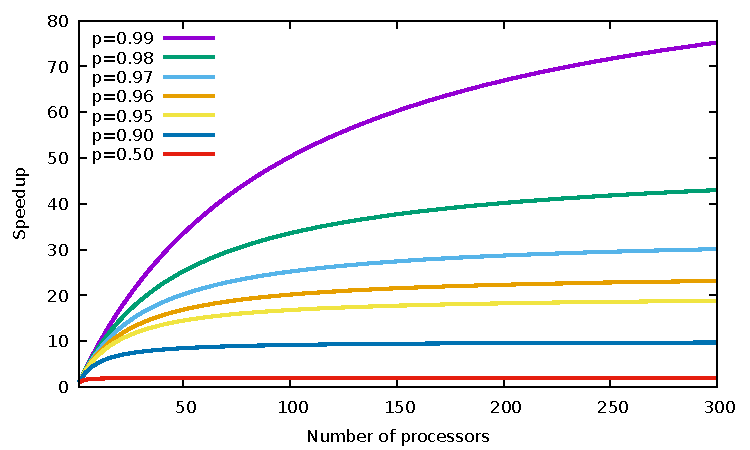
\includegraphics[width=\textwidth]{img/amdahl.pdf}
  \caption{A graph of Amdahl's Law, plotted for various values of $p$.}
  \label{fig:amdahl}
\end{figure}

\subsection{Gustafson's Law}
\label{sec:gustafson}

As parallel supercomputers became more common in the 80s, researchers
found that they routinely achieved speedup far in excess of what
Amdahl's Law would predict.  This is because Amdahl's Law is quite
pessimistic, as it assumes that the workload stays \emph{fixed} as we
gain access to more computational resources.  In practice, as
workloads increase in size, the parallelisable fraction tends to
\emph{increase} in its share of the overall runtime.  Also, when we
get access to a larger machine, we tend not to be interested in
solving our old problems faster, but in solving bigger problems in the
same time as it took to solve our old problems.  \emph{Time} is the
constant, not the workload.

Suppose we scale the runtime to be $1$ and use $s,p$ to indicate the
fraction of this unit runtime spent in sequential and parallel code
respectively on a parallel system with $N$ threads.  Then a sequential
processor would require $s+N\times{}p$ time to execute the program.
The scaled speedup of parallel execution is then

\begin{equation*}
  \frac{s+p\times N}{s+p} \\
  = s+p\times N \\
  = N + (1-N) \times s
\end{equation*}

This observation was first published by John
L. Gustafson~\cite{10.1145/42411.42415} and is therefore called
Gustafson's Law:

\begin{definition}[Gustafson's Law]\label{gustafson}
  If $s$ is the proportion of execution time that must be sequential,
  then $S(N)$ is maximum theoretical speedup achievable by execution
  on $N$ threads, and is given by

  \[
    S(N) = N + (1-N) \times s
  \]
\end{definition}

\begin{figure}
  \centering
  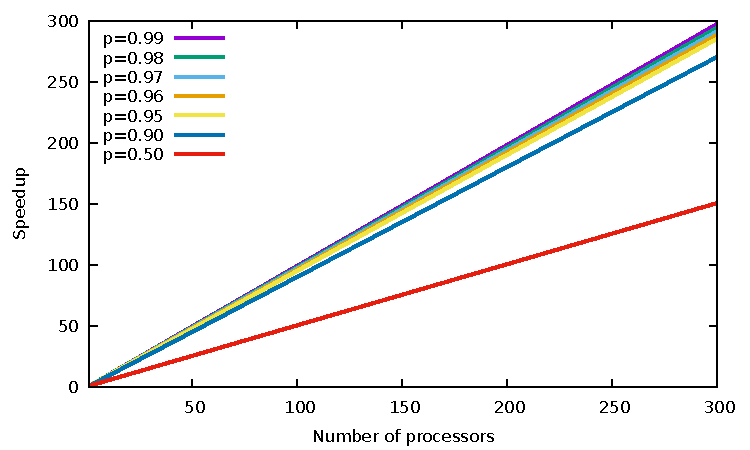
\includegraphics[width=\textwidth]{img/gustafson.pdf}
  \caption{A graph of Gustafson's Law, plotted for various values of
    $p$ (note that $p=1-s$).}
  \label{fig:gustafson}
\end{figure}

Compared to Amdahl, Gustafson is much more of an optimist---as shown
on \cref{fig:gustafson}, Gustafson's Law plots as a \textit{line},
meaning that the speedup as we add more processors is \textit{linear}.

Neither Amdahl's nor Gustafson's Laws are \emph{laws} in the common
sense of the word.  Despite providing conflicting predictions, they
can both be true under different circumstances.  Amdahl's Law tells us
about the limitations of parallelism under a fixed workload, while
Gustafson's Law tells us about the limitations of parallelism where we
assume we the workload grows proportionally with the amount of
parallelism.  Broadly, Amdahl's Law predicts strong scalability, and
Gustafson's law predicts weak scalability.

Both laws make significant simplifying assumptions---in practice,
little scientific code consists of enormous fully parallel loops with
completely independent iterations, but will tend to require some form
of routine communication, proportional to the number of processors
involved.  Specifically, these laws tend to discount the nonlinear
scaling of accessing large amounts data due to locality effects.

%%% Local Variables:
%%% mode: latex
%%% TeX-master: "notes"
%%% End:
